
\documentclass[conference]{IEEEtran}
% Windows:
% \usepackage[ansinew]{inputenc}
% Linux:
\usepackage[latin1]{inputenc}
% Mac
% \usepackage[applemac]{inputenc}
% If none of the above lines work you can also try the following:
% \usepackage[utf8]{inputenc}

\ifCLASSINFOpdf
  \usepackage[pdftex]{graphicx}
  % declare the path(s) where your graphic files are
  % \graphicspath{{../pdf/}{../jpeg/}}
  % and their extensions so you won't have to specify these with
  % every instance of \includegraphics
  % \DeclareGraphicsExtensions{.pdf,.jpeg,.png}
\else
  % or other class option (dvipsone, dvipdf, if not using dvips). graphicx
  % will default to the driver specified in the system graphics.cfg if no
  % driver is specified.
  \usepackage[dvips]{graphicx}
  % declare the path(s) where your graphic files are
  % \graphicspath{{../eps/}}
  % and their extensions so you won't have to specify these with
  % every instance of \includegraphics
  % \DeclareGraphicsExtensions{.eps}
\fi

% add custom packages
\usepackage{color}
\usepackage{hyperref}
\usepackage{algorithm}
\usepackage{algorithmic}
\usepackage{tabularx}
\usepackage{subfig}
\usepackage{mathtools}
\DeclarePairedDelimiter\ceil{\lceil}{\rceil}
\DeclarePairedDelimiter\floor{\lfloor}{\rfloor}
\definecolor{tumblue}{rgb}{0, 0.4, 0.74}
\hyphenation{op-tical net-works semi-conduc-tor}
\begin{document}
% Add the seminar's cover page
\begin{figure*}[!h]

  
\includegraphics{./images/IN.pdf} \hfill 
\includegraphics{./images/tumlogo.pdf}
 
  \vspace*{1cm}
  {\large \textsf{Fakult{\"a}t f{\"u}r Informatik}}\\
  {\large \textsf{Lehrstuhl f{\"u}r Echtzeitsysteme und Robotik}}\\
   

  \vspace*{5cm}
%
%
% TITEL DER ARBEIT
%
%
  {\color{tumblue} \Huge \bf \textsf{Clustering Similar Traffic Scenarios}}\\  % HIER EINSETZEN!

  \vspace*{1cm}
%
%
% NAME DES STUDENTEN (auf Titelblatt)
%
% 
  {\Large \bf \textsf{Murat Can \"Uste, Zhaoying Chen, Qiaoxi Liu, Emanuel Ramneantu}}\\   % HIER EINSETZEN!
 
  \vspace*{8cm}
  {\Large \textsf{Practical Course \emph{Motion Planning for Autonomous Vehicles} WS 2019/2020}}\\
 
  \vspace*{1cm} 
  \begin{tabular}{ll}
%
%
% NAME DES BETREUERS
%
%
    {\Large \bf \textsf{Advisor:}} &
    {\Large \textsf{M.Sc. Moritz Klischat}}\\                  % HIER EINSETZEN!
    \\

    {\Large \bf \textsf{Supervisor:}} &
    {\Large \textsf{Prof.~Dr.-Ing. Matthias Althoff}}\\
    \\

%
%
% ABGABETERMIN
%
%
    {\Large \bf \textsf{Submission:}} &
    {\Large \textsf{10. February 2020}}

  \end{tabular}
  
\end{figure*}
\newcommand{\algorithmautorefname}{Algorithm}
%
% paper title
% can use linebreaks \\ within to get better formatting as desired
% Do not put math or special symbols in the title.
\title{Clustering Similar Traffic Scenarios}

% author names and affiliations
% use a multiple column layout for up to three different
% affiliations
\author{\IEEEauthorblockN{Murat Can \"Uste, Zhaoying Chen, Qiaoxi Liu, Emanuel Ramneantu}
\IEEEauthorblockA{Technische Universit\"at M\"unchen\\
Email: can.ueste@tum.de, zhaoying.chen@tum.de, qiaoxi.liu@tum.de, emanuel.ramneantu@tum.de}}

\maketitle

% As a general rule, do not put math, special symbols or citations
% in the abstract
\begin{abstract}
The goal of this project is to provide a method to shutil.move(source, dest)find categories of traffic scenarios automatically. The knowledge of traffic scenario categories is important to reduce the validation and testing effort of the development of automated vehicle functions. The architecture consists of three main parts: A data generation part where datasets from different sources are converted to CommonRoad scenario format, a feature extraction part which is applied to the generated CommonRoad scenarios, a clustering technique and a classification technique applied on the extracted features. A modified unsupervised Random Forest algorithm to find a data adaptive similarity measure between all scenarios has been used in this project. The algorithm generates a path proximity matrix, which is a technique to determine similarity based on the Random Forest algorithm. This similarity matrix is then reordered with hierarchical clustering, which results in a graphically interpretable representation. It is shown how the resulting proximity matrix can be visually interpreted and how the variation of the methods' metaparameter reveals different insights into the data. The proposed method is able to cluster data from any data source that can be converted to CommonRoad scenario format. To demonstrate the methods potential, multiple features derived from highway scenarios have been used in this project.
\end{abstract}
% For peer review papers, you can put extra information on the cover
% page as needed:
% \ifCLASSOPTIONpeerreview
% \begin{center} \bfseries EDICS Category: 3-BBND \end{center}
% \fi
%
% For peerreview papers, this IEEEtran command inserts a page break and
% creates the second title. It will be ignored for other modes.
\IEEEpeerreviewmaketitle
\section{Introduction}
\IEEEPARstart
The testing and validation of automated vehicle functions take a lot of time and effort. Especially, in the case of kilometer based approach where all the conditions reqired for a given specification has to be mastered. For example, to master the specification given in \cite{shalev2017formal}, \cite{zhao2017lab}, and \cite{matthaeia2015autonomous}, billions of kilometers needs to be completed, which is not feasible. In order to overcome this, the scenario based approach is seen as a promising way to test automated vehicle functions \cite{pegasus}. However, there is an infinite number of scenarios that can appear on the road if we look at the scenarios on the microscopic level. Nevertheless, observations from higher level visualizations shows that they follow certain patterns, and can be categorized based on similarity. Therefore, there is a need to know which categories there are for the scenarios that appear on the road, which will reduce the testing and validation effort while ensuring broad scope by testing representatives from each category.

The main purpose of this project is to implement a process of categorizing/clustering of traffic scenarios in an unsupervised way. The implementation presented in this work are separated into three main parts as it can be seen on \autoref{figure:architecture}. The first part is the data generation where datasets from different sources are converted to CommonRoad scenario format \cite{althoff2017commonroad}, which provides a common format for the scenarios, as well as a benchmark for the motion planning algorithms.

\begin{figure}[!h]
  \begin{center}
  	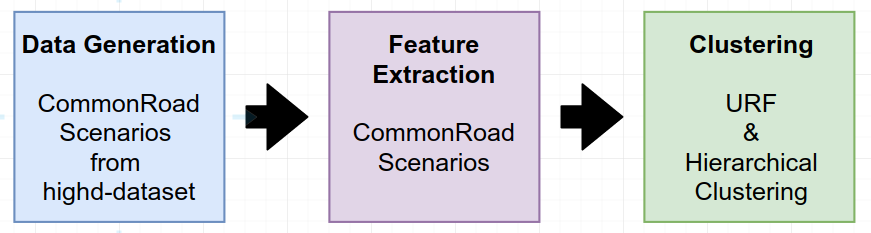
\includegraphics[width=8.5cm,height=2.3cm]{./images/proposed}
  \end{center}
  \caption{The overall architecture.}
  \label{figure:architecture}
\end{figure}

The second part is the feature extraction part where the generated CommonRoad scenarios are processed in order to create a feature model. The scenario quantitative model is inspired by the idea from \cite{Kruber2019UnsupervisedAS}. For this report, 5 specific time steps are chosen and the corresponding state of ego and surrounding vehicles are calculated.Totally 57 features are defined and implemented to describe the scenarios quantitatively. Furthermore, the importance of features is analysed, which will help feature selection in the clustering part.

Clustering is an unsupervised data exploration task. This is in contrast with supervised learning for which the datasets are labelded with classes.
We study clustering in a high dimensional numerical and categorial mixed space. The traditional methods for clustering (like kmeans clustering) have some
shortcomings. In our report, we are inspired by the idea from \cite{kruber2018unsupervised} using so called modified Unsupervised Random Forest to
 implement our algorithms as well as a handy interface to interact with raw dataset. The algorithms mainly are composed of two core techniques: 
 the clustering-based decision tree and proximity matrix (proposed in \autoref{section:forest}). 
 According to the test results from the first version of implementation,
  we notice some drawbacks and based on that we improve our algorithm.


In summary, the work presents a method which enables the clustering/categorization of scenarios from different data sources, and provides a way to investigate relations between them.

The paper is organized as follows: The data generation process, as well as the data source used are described in \autoref{section:data generation}. Then, the feature extraction process and the description of the extracted features are given in \autoref{section:feature extraction}. Afterwards, the Unsupervised Random Forest is explained in \autoref{section:forest}. Different clustering methods are presented in \autoref{section:clustering}. In \autoref{section:evaluation}, some results of the method based on the generated datasets are presented. Finally, this work is concluded in \autoref{section:conclusion}.



\section{Data generation}
\label{section:data generation}
In this section, we explain the dataset we used for this project and the data generation process in detail. 

There are several datasets with the intented purpose of traffic simulation such as NGSIM \cite{halkias2006ngsim} \cite{colyar2007us}, or automated driving research such as KITTI \cite{geiger2013vision} and Cityscapes \cite{cordts2016cityscapes}. The KITTI and Cityscapes datasets are mainly used for the development of computer vision algorithms since they contain annotated images from vehicle onboard cameras, whereas the NGSIM dataset focuses on vehicle trajectories on highways and urban traffic roads captured from bird's eye view. However, we use the highD dataset \cite{highDdataset} in this project due to the fact that even though it is similar to the NGSIM dataset as both are captured from bird's eye view and focus on highway scenarios, the highD dataset has the advantage of capturing the traffic from high longitudinal and lateral accuracy due to the usage of aerial drones, which results in lower positioning error.

The highD dataset already provides pre-extracted information about the vehicles, trajectories and important metrics. Even though these information can be used for clustering scenarios as is, we convert the highD recordings into CommonRoad scenario format \cite{althoff2017commonroad} in order to have a common format for the scenarios, and divide the recordings into small segments in order to capture traffic scenarios in the microscopic level. Another advantage of this approach would be the possibility to extend and improve the feature extraction and clustering steps later on with the usage of scenarios from wide variety of sources converted to the CommonRoad format. This would be specifically inline with the purpose of clustering and categorizing traffic scenarios in order to reduce testing and validation effort.

In the following subsections, we explain and analyze the highD dataset, and move on to the explanation of filtering and CommonRoad scenario generation processes. Lastly, we analyze the generated datasets before moving on the the feature extraction section.

\subsection{The highD Dataset}
\label{subsection:highd dataset}

The highD dataset is a dataset of naturalistic vehicle trajectories recorded on German highways. The recordings were done using an aerial drone equipped with a high resolution camera. Usage of aerial drones has the advantage of capturing the traffic from a bird's eye view with high longitudinal and lateral accuracy. Even though the information about the object heights are lost, it doesn't effect the safety validation since object heights have limited relevance. In our case, this has no effect on the resulting scenarios, since CommonRoad Scenario format also uses bird's eye view.

The recordings were done at six different highway locations in Germany around Cologne. There are total of 60 recordings, with each recording being average length of 17 minutes, which include more than 110.500 vehicles, and 147 driven hours. The road segments are about 420m length, and the number of lanes in the recordings are either 4 or 6 depending on the location, with half of them going in reverse direction compared to the other half. The datevaluationaset also contains pre-extracted information such as vehicle types, vehicle trajectories, metrics such as DHW, THW, and TTC, as well as maneuver information such as lane changes \cite{highDdataset}.

\begin{figure}[!h]
  \begin{center}
  	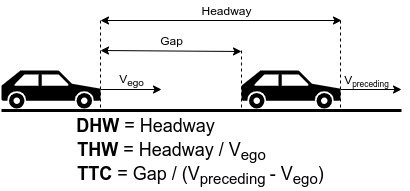
\includegraphics[width=6cm,height=2.5cm]{./images/dhw_thw_ttc}
  \end{center}
  \caption{Calculation of DHW, THW, and TTC.}
  \label{figure:dhw-thw-ttc}
\end{figure}

The DHW, THW, and TTC metrics have great importance when deciding on a scenario's criticality, and we will make use of them heavily throughout this paper. The calculation of DHW, THW, and TTC metrics are shown in \autoref{figure:dhw-thw-ttc}. The definitions of them as follows:

\begin{itemize}
	\item \textit{Distance Headway (DHW):} The distance between the front of the ego vehicle and the front of the preceding vehicle in the same lane.
	\item \textit{Time Headway (THW):} The time required for the ego vehicle's front to reach the same position as the preceding vehicle's front, if it continues with its current speed.
	\item \textit{Time to Collision (TTC):} The time required for there to be collision between the ego vehicle and the preceding vehicle, if they continue with their current speed and follow the same path.
\end{itemize}

\begin{figure}[!h]
  \begin{center}
  	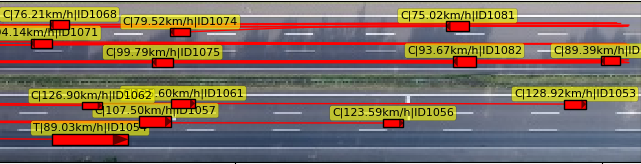
\includegraphics[width=8.5cm,height=2.5cm]{./images/highd-example}
  \end{center}
  \caption{An example segment from the highD recordings using the visualization tool provided at \cite{highdtools}.}
  \label{figure:highd example}
\end{figure} 

In \autoref{figure:highd example}, we can see an example segment from the recordings which was visualized using the tool provided at \cite{highdtools}. The red rectangles indicate the vehicles on the road, and the red lines indicate the trajectories followed by vehicles. We can also observe the vehicle type, speed of the vehicle, and the ID of the vehicle in the yellow labels.

According to \cite{highDdataset}, there are 4 main maneuvers detected on the dataset by following the rules in \cite{benmimoun2011incident} for the critical maneuvers:
\begin{itemize}
	\item \textit{Free Driving (Longitudinal uninfluenced driving):} Driving without being influenced by a preceding vehicle
	\item \textit{Vehicle Following (Longitudinal influenced driving):} Actively following another vehicle
	\item \textit{Critical Maneuver:} Low Time to Collision (TTC) or Time
Headway (THW) to a preceding vehicle
	\item \textit{Lane Change:} Crossing lane markings and staying on a
new lane 
\end{itemize}

These maneuvers were detected using predefined set of rules and thresholds. We will make use of these maneuvers during our filtering process in order to discard scenarios that pose no significant challenges to the motion planning algorithms.

\subsection{Converting highD dataset to CommonRoad Scenarios}
\label{subsection:converting highd to commonroad}
In order to convert highD recordings to CommonRoad Scenarios, we inpect each vehicle with their trajectories and consider the most critical maneuver performed by the vehicle as a scenario candidate during the conversion process. The order of criticality is as follows; the \textit{Lane Change} maneuver is more critical then \textit{Critical Maneuver}, followed by \textit{Vehicle Following} and then \textit{Free Driving}. 

In \autoref{figure:raw dataset maneuver statistics}, we can see the percentages of the mentioned maneuvers performed by vehicles after assigning each vehicle to its most critical maneuver group. The \textit{Lane Change} maneuvers are filtered based on the number of lane changes defined for the vehicles in the dataset, which means we select the vehicles that performed at least one lane change during the recording. The vehicles with no \textit{minimum DHW} defined were assigned to the group of \textit{Free Driving} maneuvers. The vehicles that didn't perform any lane changes, and had \textit{minimum DHW} defined were assigned to the \textit{Vehicle Following} and \textit{Critical Maneuver} groups, where the latter group having \textit{minimum THW} lower than 1.75 seconds and/or \textit{minimum TTC} lower than 0.5 seconds. These thresholds were taken from \cite{benmimoun2011incident}, as the highest thresholds for a scenario to be identified as a \textit{critical maneuver}.\\ 

\begin{figure}[!h]
  \begin{center}
  	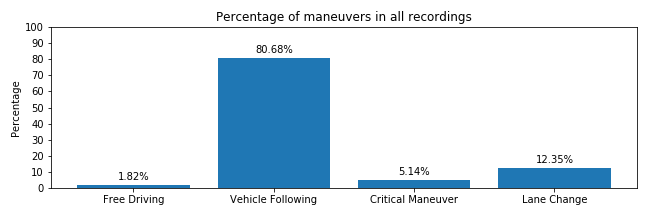
\includegraphics[width=8.5cm,height=3cm]{./images/raw_maneuvers}
  \end{center}
  \caption{Percentage of detected maneuvers on the highD dataset.}
  \label{figure:raw dataset maneuver statistics}
\end{figure}

One thing to note here is that, the DHW, THW, and TTC metrics were calculated without a distance threshold in the dataset. If we apply a distance threshold in the dataset, for example a sensor range, the percentages of the maneuvers on \autoref{figure:raw dataset maneuver statistics} would change drastically, moving significant portion of \textit{Vehicle Following} group over to the \textit{Free Driving} group. 

Since the \textit{Free Driving} scenarios pose no significant challenge to the motion planning algorithms, we try to filter out as much of them as possible, and increase the percentage of other critical maneuvers. In order to do so, we apply a filtering process on the data before we move on to the actual scenario generation.\\

\subsubsection{Filtering Process}
\label{subsubsection:filtering process}
As mentioned before, we inspect each vehicle and their trajectories in the dataset and consider their most critical maneuver as a candidate for a scenario. This is done by the usage of metrics DHW, THW, and TTC, as well as the lane change information of the vehicles. Following steps are performed on each recording to filter out critical scenarios based on lane change information and one of the DHW, THW, or TTC metrics of each vehicle:

\begin{itemize}
	\item \textit{Step 1:} Filter out trajectories that don't have the selected metric defined.
	\item \textit{Step 2:} Filter out trajectories that don't perform lane change maneuver if we want to use the lane changing vehicles only.
	\item \textit{Step 3:} Sort each trajectories' frames based on selected metric, and select the time step with minimum value for each trajectory.
	\item \textit{Step 4:} Generate the scenarios by setting the selected time steps as the middle time step of a scenario.
\end{itemize}

We decided to have total of 81 time steps in our generated scenarios, which will result in 3.24 seconds long segments. Since the recordings have 25 frames per second, the $\Delta time$ between each time step is 0.04 seconds. The timespan of 3.24 seconds, or 81 time steps, was decided after visualizing the extracted scenarios, and observing that in most of the scenarios, the maneuvers performed by the ego vehicle (i.e lane change) was finalized within this time span. 

To give an example of a filtering process, we can select DHW metric for criticality, and use only the lane changing tracks. After we filter out the tracks that don't have the DHW metric defined, and don't perform lane changes during the recording, we would be left with a subset of vehicles from the recording. Afterwards, we would sort each vehicles' trajectory states based on dhw metric, and select the time step with the lowest DHW value for each vehicle. Each of these vehicles, and their corresponding time steps, would be the ego vehicle of a scenario, and the middle time step of the scenario respectively, if they are not discarded during the scenario generation process.

After selecting the most critical time step for each vehicle in the recordings after filtering, we move on to the CommonRoad Scenario generation process.
\\

\subsubsection{CommonRoad Scenario Generation Process}
\label{subsubsection:scenario generation process}
After the filtering process is done, we are left with sets of vehicles and their most critical time steps for each recording. Setting the associated time steps as the middle time steps of the scenario candidates, we calculate the initial and final time steps of the scenario by going 40 frames back, and forward in the recording. Afterwards, we inspect the segment between these frames of the recordings to discard scenario candidates that are not fit to be converted to CommonRoad scenario format. The main steps of scenario generation as follows:

\begin{itemize}
	\item \textit{Step 1:} Discard the scenario if there are not enough time steps for the selected trajectory when the associated frame is selected as the middle time step.
	\item \textit{Step 2:} Discard the scenario if the initial or final position of the ego vehicle is too close to the scenario's edges, in order to have meaningful features during the feature extraction process.
	\item \textit{Step 3:} Discard the lanelets and trajectories that are in the opposite direction. Since the lanelets in opposite directions are physically seperated, they have no effect on the scenario, and would provide unnecessary information.
	\item \textit{Step 4:} Generate dynamic obstacles from all vehicles within the
selected initial and final time steps.
	\item \textit{Step 5:} Set the obstacle ID of the dynamic obstacle that corresponds to the ego vehicle to a unique number in order to differantiate it from rest of the obstacles (99 was assigned in our case).
\end{itemize}

As it can be seen, we look whether the selected vehicle has enough time steps in its trajectory for the defined segment, and whether its initial and final time step positions are too close to the scenario's edges. The positional check is done in order to make sure we can extract meaningful features during the feature extraction process. This will be explained in detail on \autoref{section:feature extraction}.

Additionally, we remove the dynamic obstacles within the defined segment if they don't have at least 10 time steps defined in their trajectories. This means that, the vehicles go out of the scenario during the inital time steps, or come into the scenario during the final timesteps are dicarded, since they have no effect on the scenario and have very little information.

\subsection{Generated CommonRoad Scenario Datasets}
\label{subsection:generated commonroad datasets}
After applying the filtering and scenario generation processes to the highD dataset with three different metrics and two different cases of including only lane changing vehicles, and including all vehicles on the dataset, we generated 6 different CommonRoad scenario datasets. Including only the lane changing tracks during generation of scenarios results in smaller datasets since we are only considering 12.35\% of the vehicles in the dataset as it can be seen on the \autoref{figure:raw dataset maneuver statistics}. In the case of including all vehicles, we end up using 98.18\% of the vehicles on the dataset. Since we are filtering out the vehicles where the selected metric was not defined, the \textit{Free Driving} scenarios are being filtered out as they are not following a preceding vehicle, meaning that none of the metrics are defined for them.\\

\begin{table}[!h]
	\centering
    \caption{Generated CommonRoad Scenario Datasets}
    \begin{tabularx}{\columnwidth}{|X||X|X|X|}
 		\hline
 		Dataset Name & Metric & Only Lane Changing & Sample Size\\
 		\hline
 		DHW Small & Min DHW & True  & 6.551\\
 		THW Small & Min THW & True  & 6.544\\
 		TTC Small & Min TTC & True  & 6.944\\
 		DHW Big   & Min DHW & False & 44.812\\
 		THW Big   & Min THW & False & 44.107\\
 		TTC Big   & Min TTC & False & 44.280\\
 		\hline
	\end{tabularx}
	\label{table:generated datasets}
\end{table}

We can see the combination of parameters used for filtering, and the resulting dataset sizes in \autoref{table:generated datasets}. As the datasets generated using only the lane changing tracks result in having a smaller set of generated dataset, we named them by appending 'Small' after the selected metric's name. And similarly we named the datasets generated using all vehicles by appending 'Big' after the selected metric's name.

The number of scenarios generated for the small datasets are 6.680 on average, which means that we are discarding at least half of the scenarios during the filtering and scenario generation processes, as the number of vehicles that performs \textit{Lane Change} maneuver should be around 13.647 (there are 110.500 vehicles in the dataset, 12.35\% of them are performing \textit{Lane Change} maneuver).

The number of scenarios generated for the big datasets are 44.400 on average, which means that we are discarding more than half of the scenarios during the filtering and scenario generation processes, as the number of vehicles should be around 108.489 excluding the \textit{Free Driving} maneuver vehicles (there are 110.500 vehicles in the dataset, and we consider 98.18\% of them).

In \autoref{figure:generated scenario}, we can see two examples of a generated CommonRoad scenarios. Both of these scenarios were taken from the dataset that was generated using TTC as metric, and only lane changing vehicles. The figures show each scenario's most critical time step (41st time step) based on the ego vehicles. In Figure \autoref{figure:generated scenario:vehicle following}, the vehicle performs the \textit{Vehicle Following} maneuver throughout the scenario, and the figure shows the \textit{minimum TTC} time step for the ego vehicle. In Figure \autoref{figure:generated scenario:lane change}, the vehicle performs the \textit{Lane Change} maneuver, and the figure shows the \textit{minimum TTC} time step for the ego vehicle. In both cases, the lanes and vehicle going in reverse direction were removed from the scenario.

In order to inspect the generated datasets in detail, we analysed the maneuvers in each dataset in a similar manner to the \autoref{figure:raw dataset maneuver statistics} using the same set of rules and thresholds after the feature extraction was performed on all of them.

\begin{figure}[!h]
  \begin{center}
  	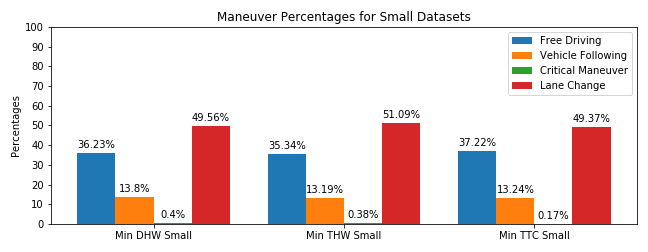
\includegraphics[width=8.5cm,height=3.7cm]{./images/small_datasets_maneuvers}
  \end{center}
  \caption{Percentage of the detected maneuvers on the generated datasets with considering only lane changing vehicles.}
  \label{figure:small dataset maneuvers}
\end{figure}

In \autoref{figure:small dataset maneuvers}, we can see the percentages of detected maneuvers on each small datasets. Even though the vehicles that performed \textit{Lane Change} maneuver were selected for the generation of the small datasets, the resulting maneuvers are not all \textit{Lane Change} maneuvers. This means that even if the vehicle performs a lane change, its most critical time step in terms of the selected metric might not necessarily be during the lane change maneuver.

\begin{figure*}[!h]
\centering
\subfloat[An example of \textit{Vehicle Following} maneuver on the generated datasets.]{
	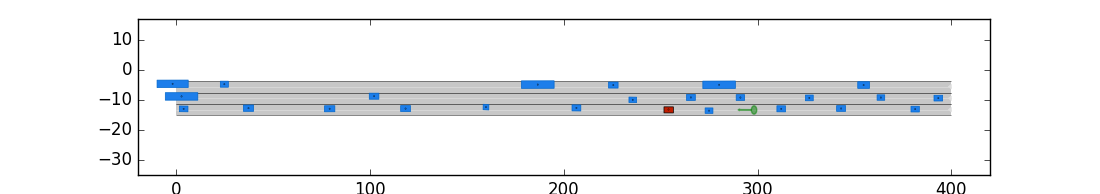
\includegraphics[width=6in]{./images/vehicle_following_example}%
	\label{figure:generated scenario:vehicle following}
}
\vfill
\subfloat[An example of \textit{Lane Change} maneuver on the generated datasets.]{
	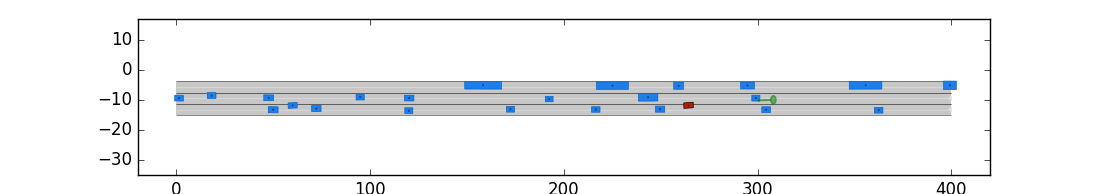
\includegraphics[width=6in]{./images/lane_change_example}%
	\label{figure:generated scenario:lane change}
}
\caption{Visualization of two examples from the generated dataset with TTC as the metric, and considering only the lane changing vehicles. The figures show each scenario's most critical time step based on the ego vehicle. In (a) we can see an example of \textit{Vehicle Following} maneuver, whereas in (b) we can see an example of \textit{Lane Change} maneuver performed by the ego vehicle.}
\label{figure:generated scenario}
\end{figure*}

Other important difference in the ratio of the maneuvers is that the ratio of \textit{Free Driving} maneuver is a lot higher compared to before. This is the result of applying a distance threshold in order to simulate sensor range during the feature extraction process, meaning that the \textit{Vehicle Following} and \textit{Lane Change} maneuvers where the preceding vehicle is outside of the sensor range (100 meters in our case) are considered as \textit{Free Driving} from ego vehicle's perspective.

\begin{figure}[!h]
  \begin{center}
  	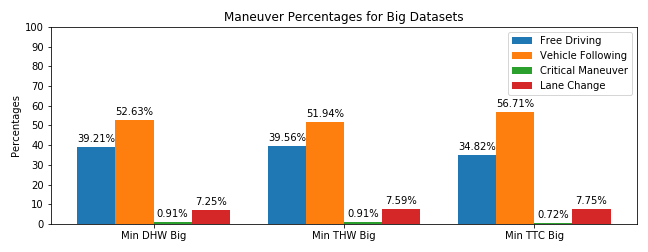
\includegraphics[width=8.5cm,height=3.7cm]{./images/big_datasets_maneuvers}
  \end{center}
  \caption{Percentage of the detected maneuvers on the generated datasets with considering all vehicles except the ones with \textit{Free Driving} maneuver.}
  \label{figure:big dataset maneuvers}
\end{figure}

Similarly, in \autoref{figure:big dataset maneuvers}, we can see the percentages of detected maneuvers on each big datasets. In this case the ratio of each maneuver is similar to the original dataset, except the \textit{Free Driving} maneuvers, which was caused by the distance threshold explained above, which results in having lower ratio for \textit{Vehicle Following} and \textit{Lane Change}.

Another thing to notice here is that the ratio of \textit{Critical Maneuver} is much lower in all datasets compared to the original. This is due to the scenario generation process where we discard scenarios where there are not enough time steps in the ego vehicle's trajectory, and the position of the inital or final state of the ego vehicle being too close to the edges.

\section{Feature extraction}
\label{section:feature extraction}
The main purpose of feature extraction is to extract typical characteristics of the scenarios and build a quantitative model for them. Based on the actual highway model, the area around the ego is divided into six zones and we apply a sensor range of the ego vehicle (100 meters in our case). It is assumed that only the vehicles inside the sensor range of ego vehicle would influence the maneuver of ego vehicle and only the nearest surrounding vehicles on or next to the lane where ego vehicle is would directly influence the ego vehicle. The proposition is depicted in Figure \ref{fig:ScenarioModel}.

\begin{figure*}[!h]
  \centering
  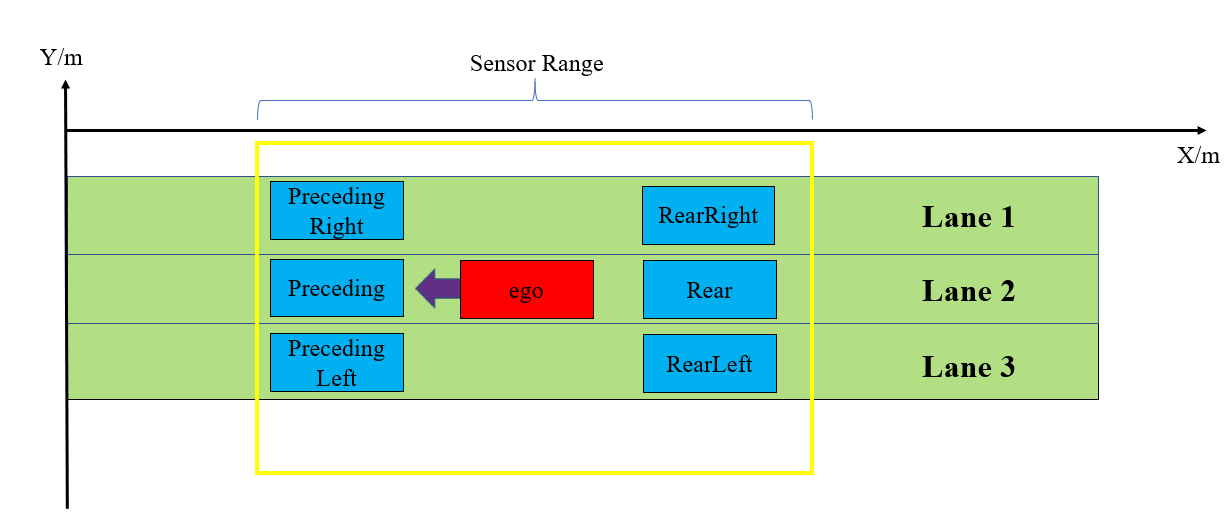
\includegraphics[width=6in]{./images/ScenarioModel.png}
  \caption{Only the surrounding vehicles (preceding right, preceding, preceding left, rear right, rear and rear left vehicles) in the sensor range (yellow box) are considered in the scenario model. In our paper, the size of sensor range is 100 meters.}
  \label{fig:ScenarioModel}
  \end{figure*}
  

\subsection{Feature Model}
As mentioned before, the minimal THW, DHW and TTC are the metrics to determine the criticality of scenarios, because the states of vehicles represent more typical characteristic of scenarios at these timesteps. Therefore, the features are set up on five timesteps: At the beginning, the minimal THW, the minimal DHW, the minimal TTC and the end. To describe the traffic density, we consider the relative distance between ego vehicle and its surrounding vehicles. Also, we calculate how many surrounding vehicles there are.

Other features are defined according to the state of ego vehicle and we observe its changes over time. On one hand, we keep record some basic states of ego vehicle including acceleration and absolute velocity. On the other hand, we consider its three typical maneuvers, including lane change, cut-in and brake to describe the mainly moving pattern of the ego vehicle and further describe the characteristics of the scenarios.

In total a set of 57 features are defined and calculated to be fed in the clustering process. The feature structure is shown in Figure \ref{fig:FeatureSturcture}. The description of all features is in the appendix.

\begin{figure*}[!h]
  \centering
  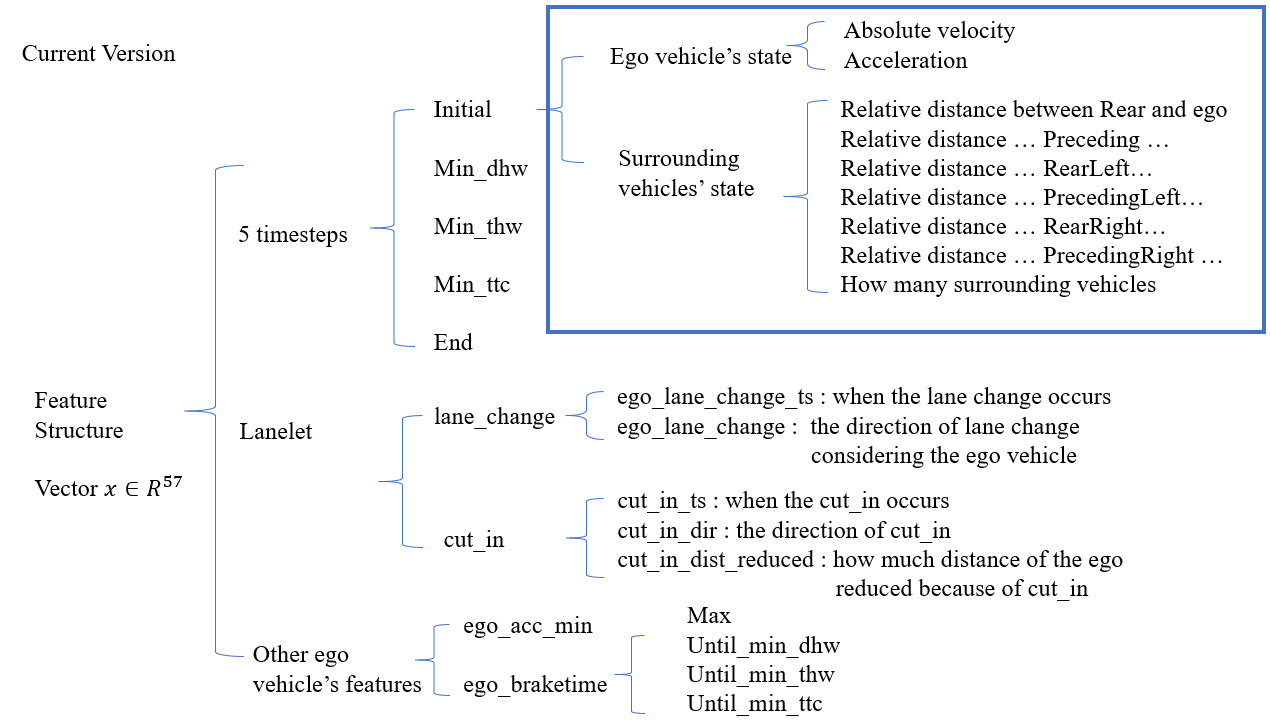
\includegraphics[width=6in]{./images/CurrentVersion.png}
  \caption{The feature structure.}
  \label{fig:FeatureSturcture}
  \end{figure*}


\subsection{Analysis of Crucial Features}
A feature vector can include all the 57 features to describe a scenario. However, it will be time-consuming when clustering because some relatively less important features are considered. To strike a balance between describing the scenarios accurately and decreasing the computation when clustering, we need to analysis the crucial level of certain kinds of features. After we know which features are more crucial, we can only choose those features to form a feature vector used in the clustering part.

Based on the Random Forest algorithm, when splitting trees, we choose the features with highest \textit{Gini Gain} as the splitting feature. The more frequent a feature is chosen, the more important it will be. We take an experiment in the dataset with \textit{dhw-only-lanchanging} metric, building 300 trees with maximal depth of tree = 5. The Figure \ref{fig:BarChart_Feature--times} shows the statistics about how many times that each feature to be chosen.

\begin{figure}[!h]
  \centering
  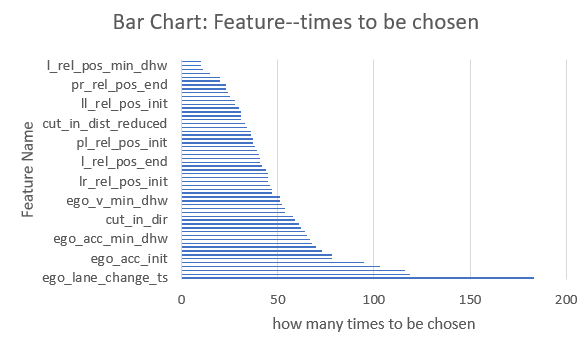
\includegraphics[width=8.5cm,height=3.7cm]{./images/BarChartFeatureTimes.png}
  \caption{There are totally 2814 splits. The most frequently chosen feature is \textit{ego-lane-change-ts} (when the ego lane change occurs) with 183-time chosen and the less frequently chosen feature is the relative position between rear vehicle and ego vehicle at minimal dhw, with 10-time chosen.}
  \label{fig:BarChart_Feature--times}
  \end{figure}
  
We separate the relative features into various groups and calculate the average chosen times of each group of features. 7 groups are defined as shown in figure \ref{fig:analysis_crucial_features}.
  
\begin{figure}[!h]
  \centering
  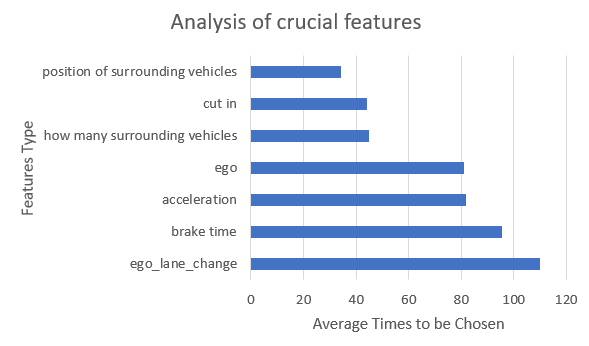
\includegraphics[width=8.5cm,height=3.7cm]{./images/AnalysisCrucialFeatures.png}
  \caption{The average chosen times of each grouping features. }
  \label{fig:analysis_crucial_features}
  \end{figure}

The order of crucial features is as follows:
\begin{itemize}
    \item Compared the state of ego vehicle:\\ego lane change \textgreater brake time\textgreater acceleration\textgreater cut in
    \item Compared the state of ego vehicle and its surrounding vehicles:\\
ego vehicle's state\textgreater  surrounding vehicles' state
\end{itemize}

Thus, if we need to decrease the size of feature vector for faster computation, we can ignore certain features based on the statistics. Specially, the relative position of the surrounding vehicles is less crucial.
% An example of a floating figure using the graphicx package.
% Note that \label must occur AFTER (or within) \caption.
% For figures, \caption should occur after the \includegraphics.
% Note that IEEEtran v1.7 and later has special internal code that
% is designed to preserve the operation of \label within \caption
% even when the captionsoff option is in effect. However, because
% of issues like this, it may be the safest practice to put all your
% \label just after \caption rather than within \caption{}.
%
% Reminder: the "draftcls" or "draftclsnofoot", not "draft", class
% option should be used if it is desired that the figures are to be
% displayed while in draft mode.
%
%\begin{figure}[!t]
%\centering
%\includegraphics[width=2.5in]{myfigure}
% where an .eps filename suffix will be assumed under latex, 
% and a .pdf suffix will be assumed for pdflatex; or what has been declared
% via \DeclareGraphicsExtensions.
%\caption{Simulation Results.}
%\label{fig_sim}
%\end{figure}

% Note that IEEE typically puts floats only at the top, even when this
% results in a large percentage of a column being occupied by floats.


% An example of a double column floating figure using two subfigures.
% (The subfig.sty package must be loaded for this to work.)
% The subfigure \label commands are set within each subfloat command,
% and the \label for the overall figure must come after \caption.
% \hfil is used as a separator to get equal spacing.
% Watch out that the combined width of all the subfigures on a 
% line do not exceed the text width or a line break will occur.
%

\begin{figure*}[!t]
\centering
\subfloat[first cut]{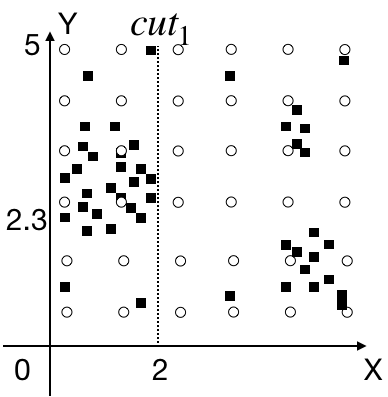
\includegraphics[width=1.6in]{./images/splitdemo1}%
\label{first}}
\hfil
\subfloat[clean synthetic data]{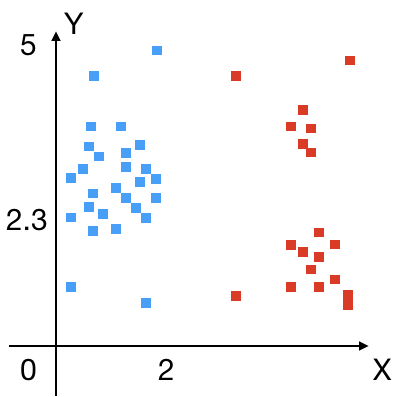
\includegraphics[width=1.6in]{./images/splitdemo2}%
\label{second}}
\hfil
\subfloat[second cut]{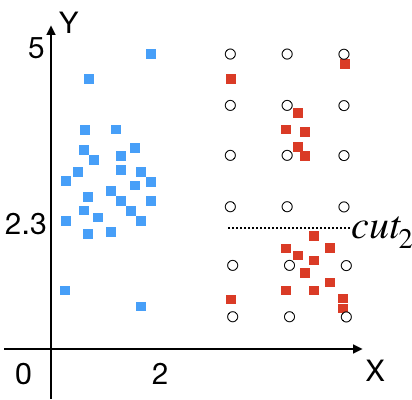
\includegraphics[width=1.6in]{./images/splitdemo3}%
\label{third}}
\hfil
\subfloat[final cluster result]{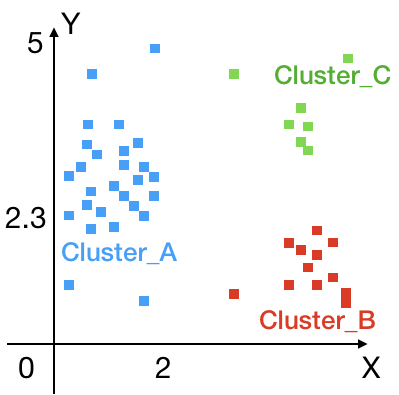
\includegraphics[width=1.6in]{./images/splitdemo4}%
\label{forth}}
\caption{Simulation of generating synthetic data and splitting on two dimensional data. (a) shows the first split by feature X at the value 2. 
Because on the left of $cut_1$, it has a majority of black points whereas on the right side it has more white points. 
Finished first split, white points are deleted. the process for second split by feature Y is similar as the first. After two times split, all the datapoints are loacted in one cluster.}
\label{fig_sim}
\end{figure*}
%
% Note that often IEEE papers with subfigures do not employ subfigure
% captions (using the optional argument to \subfloat[]), but instead will
% reference/describe all of them (a), (b), etc., within the main caption.


% An example of a floating table. Note that, for IEEE style tables, the 
% \caption command should come BEFORE the table. Table text will default to
% \footnotesize as IEEE normally uses this smaller font for tables.
% The \label must come after \caption as always.
%

\section{Unsupervized Random Forest}
\label{section:forest}
The aim of our task is to cluster similar traffic scenarios in an unlabeled dataset. 
As mentioned before, we defined more than 50 features on the data set which is high dimentional.
Furthermore, the dataset also have different types of data, namely, numerial and categorial. 
Besides, the data also varies according to the feature. Therefore, we apply the idea from random forest (RF) to group the relevant scenarios.
Since the classical application of RF is introuduced for supervised learning, it leads to a similarity measurement between labeled classes.
\cite{shi2006unsupervised} shows that RF predictor also works on unlabeled data well by generating synthetic data. Here we describe the properties of unsupervised RF method and how we implement 
for clustering traffic sccenarios in practice.
\subsection{Motivation of Random Forest(RF)}
RF is a well known ensemble predictor of individual classification tree predictors. The URF method distinguishing the original data from the synthetic data yields a similarity
measure that can be used as input in further unsupervised learning algorithms. The basic principle is, each tree votes for a classification and the forest chooses the classification which has the most votes over all the trees.
Compared with tranditional RF, the difference of URF is constructing each binary decision tree by adding an argumented dataset as labeled datapoints.
Advantages of URF:
\begin{itemize}
  \item It can handle mixed variables (numerical and categorial).
  \item It gives estimate of which features are important. (explainable for feature engineering)
  \item As ensemble learning method, it reduces overfitting and maintains robust for missing data and outliers.
  \item It computes proximities between pairs of cases that can be used in clustering.
  \end{itemize}
\subsection{Challenges of classical RF}
\subsubsection{Unlabeled dataset}\label{challenge1}
However,the main problem of URF is: If the original data distributed in high dimensional spaces is not dense or well balanced, based on this, Generating synthetic data leads to an exponential number of synthetic datapoints.\cite{kruber2018unsupervised}
In order to overcome the drawback of URF, a method called CLustering Tree (CLTree) is introduced in \cite{liu2000clustering}
\\Instead of adding augmented dataset in fully dimensional space, the CLTree technique creates uniformly distributed points in each split where only one feature (one dimension) determines the splitting result.
Inspired by CLTree, we impemented our Modified URF algorithm in Python for our clustering scenarios task based on constructing decision tree for the binary classification.
\subsubsection{Similarity Measurement}
After detecting a URF clustering result, we have to consider how (dis)similar among them. For labeled dataset, the terminal leaves in which the datapoints are landed are considered. If two obeservations placed in the same leave node, during accumulating the result of forest, the similarity between them is increased by one. 
Finally, the average similaries between each pair of datapoints is calculated and can be applied for further distance measurement. 
In \cite{Kruber2019UnsupervisedAS} a proximity measure was introduced. Intuitively, each scenario starting from the root node, went through some decision node and at the end arrived a leave node. 
The whole journey of one datapoint reflect the property of this datapoint since each decision node has its criterion feature and corresponding value. Thus, the difference between two datapoints is the different path they traveled.
The more overlapped nodes they passed by, the more common properties they have, the more similar they are. Concrete solution is illustrated later in \autoref{proximitysection}
\subsection{Solution and Implementation}
This part presents how we apply modified URF algorithm by generating synthetic data as well as similarity measurement method in practice to achieve our goal. 
\subsubsection{modified Decision Tree (DT) Construction}
As mentioned in \autoref{challenge1}, in order to transfer our unsupervised task (clustering ) into a supervised method, our goal turns to separate synthetic from original data. 
Since it is principally a decision tree which perform a binary split, we modify the algorithm and use Gini purity as splitting criterion.\\
In python we define a Class $DecisionNode$ which is the component of a tree. It has several attributes: the splitting feature, the splitting value, the result which could be another $DecisionNode$ or a dictionary composed of clustered points.
\\\\The input for a DT in our task is a set of artificially labeled datapoints which consists of two part: scenearios from original dataset (labeled as 0) and synthetic points uniformly generated.
\\\\A decision tree has two types of nodes, decison nodes ($DesicionNode$) and leaf nodes (the dictionary stored in its $DesicionNode$'s result). A decison node which can also regarded as subtree includes the decision feature and two branches.
Thus we can build a tree recursively: (See \autoref{dt})
\begin{algorithm}[!h]
	\caption{BuildTree$(df,mLeaves,gini,minMax,col)$}
  \label{dt}
  \begin{algorithmic}[1]
    \IF{$length(df)==0$}
     \STATE {$DecisionNode()$}
      \IF{$length(df)>mLeaves$}
      \STATE $createfakeData(df,minMax,col)$
       \STATE $selectLocalBestGini$
       \STATE $selectGlobalBestGini$
       \STATE $bFea,sValue,bGini <- selectGlobalBestGini$
        \IF{$bGini>=gini$}
         \STATE $set1,set2 <- split(df,bFea,sValue)$
         \STATE $branch1 <- BuildTree(set1,..)$
         \STATE $branch2 <- BuildTree(set2,..)$
         \RETURN {$DecisionNode()$}
        \ENDIF
        \RETURN {$DecisionNode()$}
      \ENDIF
    \ELSE
    \RETURN {$DecisionNode()$}
    \ENDIF
	\end{algorithmic}
\end{algorithm}

\begin{figure}[!h]
  \begin{center}
  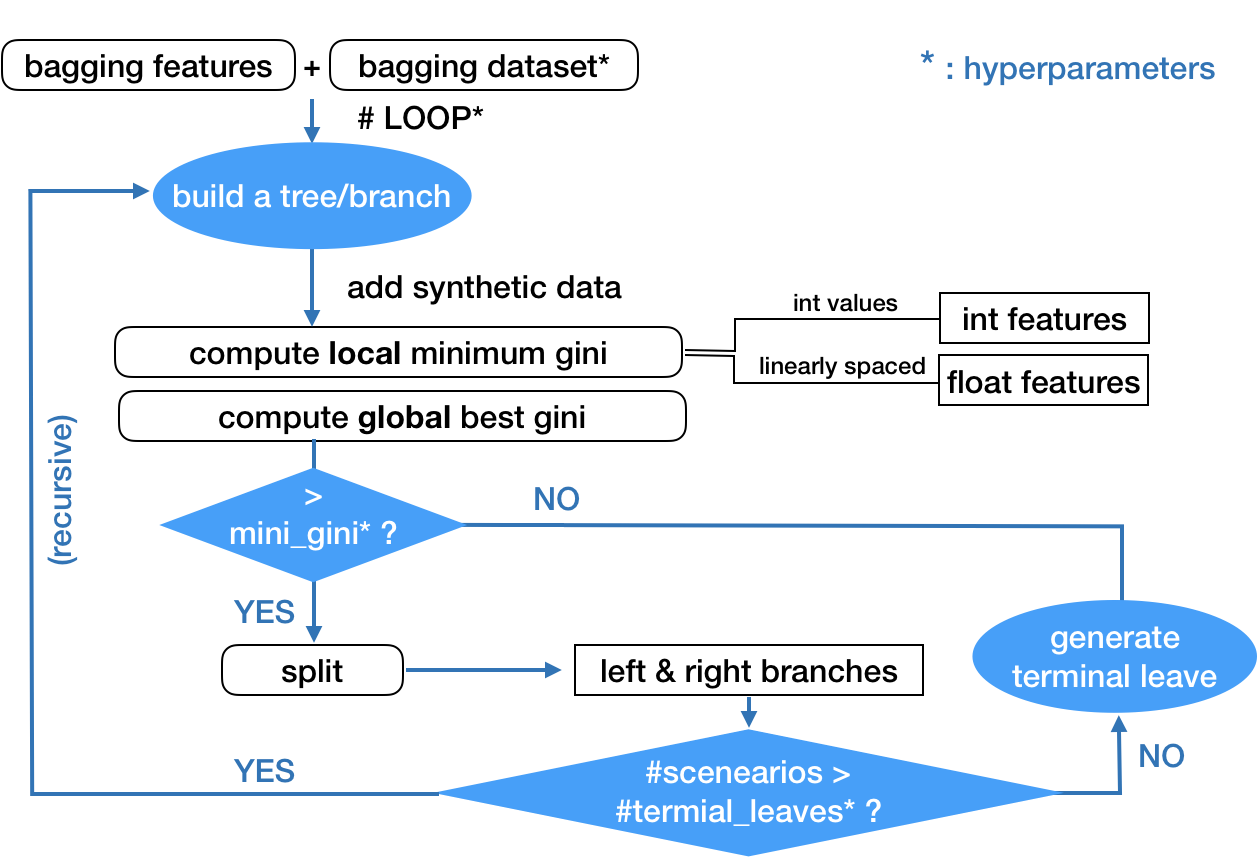
\includegraphics[width=8.5cm,height=6cm]{./images/decisiontree_diagram}
  \end{center}
  \caption{Diagram of Modifed URF Algorithm}
  \label{MURF}
  \end{figure}
  \begin{enumerate}
    \item Initial state: N obeservations with M features, number of datapoints becoming a leaf (for pruning) is L.
    \item Sample $r*N$ obeservations randomly (ratio $r$ is a hyperparameter) with replacement and select randomly $m=\floor*{\sqrt{M}}$ number of features $f_1,f_2,..f_m$.
    \item If the number of datapoints is smaller than L, Stop growing.
    \item Generate synthetic data (uniformly distributed) randomly for each selected feature dimension by the minimum and maximum values over original data ranges.\cite{kruber2018unsupervised}
    \item Calculate best split value $bs_i$ using Gini index as splitting criterion for each chosen feature $f_i$.
    \item Compare with all best split values of features and choose $bValue =min(bs_1,...,bs_m)$ as the global best split value as well as corresponding feature $f_{split}$
    \item Deleted all synthetic data and divide dataset by $f_{split}$ and $bValue$ into left and right branch. 
    \item loop back to the third step.
    \end{enumerate}
  \subsubsection{Preorder Tree Traversal}
  After constructing the most important conponement,the individual DT, we start to implement the complete URF algorithm.
  \\The root node ($DecisionNode$) of each tree in the forest contains a bootstrap sample from the original data as the training set. The leave nodes belonging to their parent $DesicionNode$ store the clustered datapoints.
  That is to say, in order to apply the result of a DT for statistic, we write a recursive function $PreTraversal$ which is responsible for pre-order tree traversal. The algorithm which has only three basic steps is consise combined with our self-defined class $DesicionNode$. (See \autoref{traversal})
  The input is a $DecisionNode$ which can either a tree or a subtree while output is a dictionary in which the key is the unique datapoint ID and the corresponding path (defined in \autoref{proximitysection}) is the value. 
  Main steps on $PreTraversal$ are as following:
  \begin{enumerate}
    \item visit the node, check wether it is a leave node. If not, then continue; Otherwise return the stored datapoints, End.
    \item visit its left branch (recursively)
    \item visit its right branch (recursively)
    \end{enumerate}
  \begin{algorithm}[!h]
    \caption{PreTraversal$(tree,pos,res,depth=0)$}
    \label{traversal}
    \begin{algorithmic}[1]
      \IF{$tree.value!= None$}
      \STATE $pos_l = pos + 'L' $
      \STATE $pos_r = pos + 'R' $
      \IF{$tree.left.res!= None$}
      \STATE $res[pos_l] = tree.left.res$
      \ENDIF
      \IF{$tree.right.res!= None$}
      \STATE $res[pos_r] = tree.right.res$
      \ENDIF
      \STATE$PreTraversal(tree.left,depth+1,pos=pos_l,res)$
      \STATE$PreTraversal(tree.right,depth+1,pos=pos_r,res)$
      \ELSE
      \STATE $res[pos] = tree.res$
      \ENDIF
      \RETURN {$res$}
    \end{algorithmic}
  \end{algorithm}
  \begin{figure*}[!t]
    \centering
    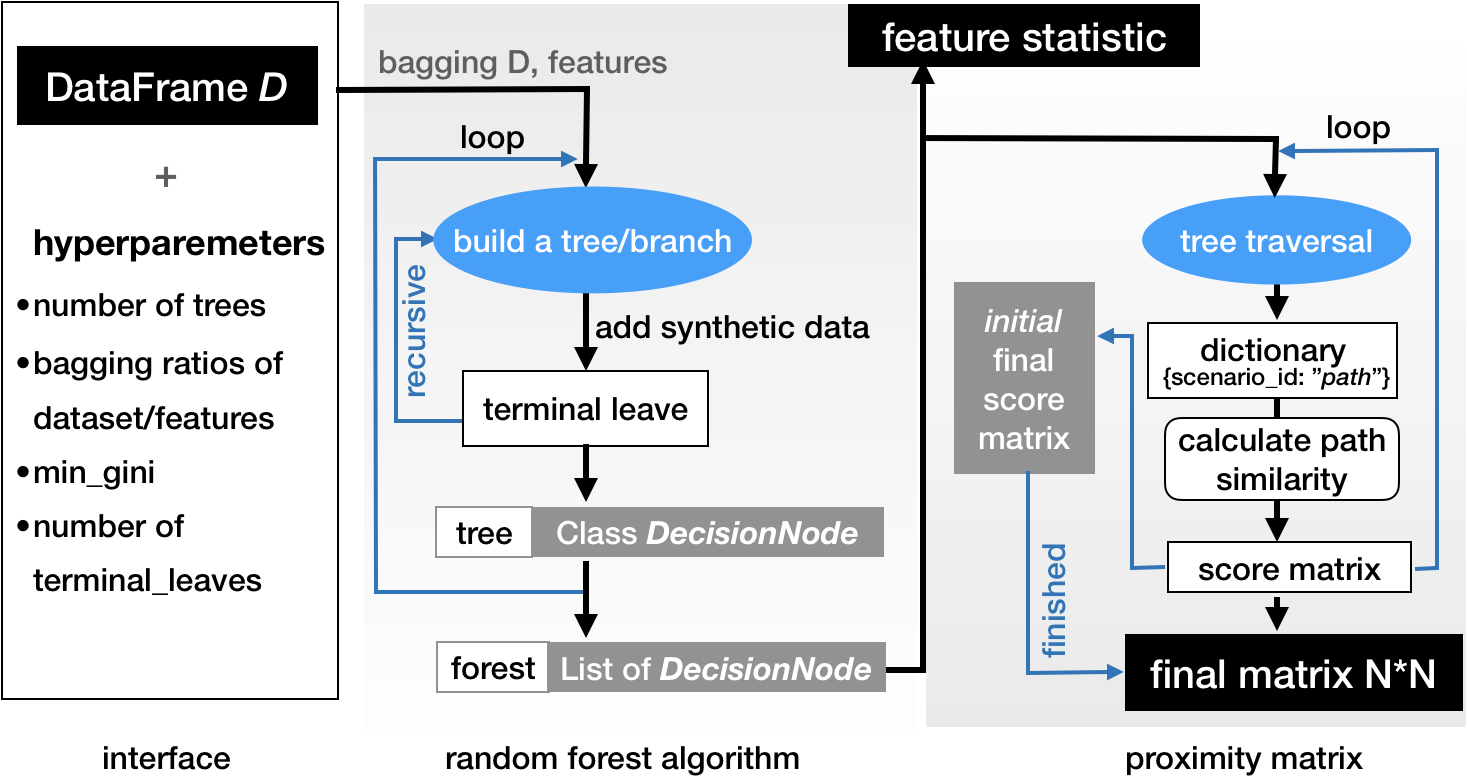
\includegraphics[width=5in]{./images/diagram}
    \caption{An Overview of the Implementation from dataset to proximity matrix}
    \label{overview}
    \end{figure*}
\subsubsection{Implementation of Proximity Matrix }\label{proximitysection}
Since we yield a forest according to modified URF, datapoints(scenarios) are landed in multiple trees.
\\
\begin{figure}[!t]
  \centering
  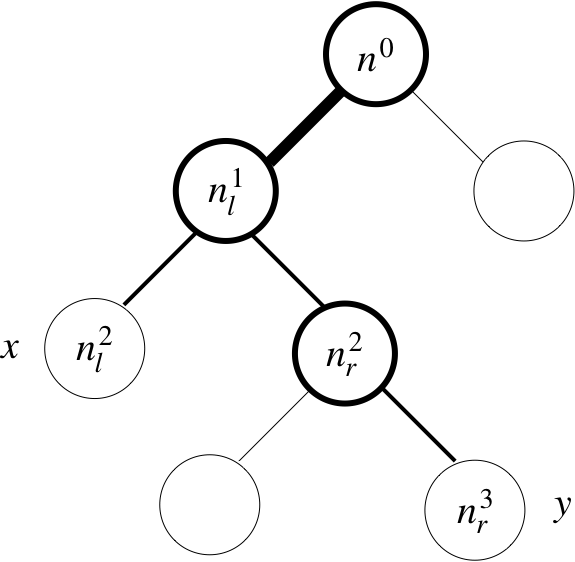
\includegraphics[width=1.5in]{./images/path}
  \caption{Example of the proximity path from a pair $(x,y)$ where $x$ located in leave node $n^2_{l}$ while y in $n^3_{r}$. $p_{x}=\{n^0, n^1_{l}, n^2_{l}\}$, $p_{y}=\{n^0, n^1_{l}, n^2_{r}, n^3_{r}$\}. 
  Thus in this tree $score_{x,y}=\frac{2}{5}$ }
  \label{fig_sim}
  \end{figure}
In the forest, a tree $T^k$ is built based on our dataset $D$. We define a path of a datapoint (scenario) $x$ in $T^i$ through all decision nodes as 
$$p^k_{x}=\{n^0, n^1_{pos},...,n^m_{pos},\}$$ where $pos$ is either left or right, $m$ represents the depth of this tree.\\
In our work, we apply Jaccard Index for calculating the similarity score between pair of datapoints $x$ and $y$. Namely,
$$score_{x,y}(T^k) = \frac{|p^k_{x} \cap p^k_{y}|}{|p^k_{x} \cup p^k_{y}|} \in (0,1]$$
Because of ensemble predictor, at the end we need average all trees in the forest. 
Assume that the pair of $x$ and $y$ appears N times in N trees, the final proximity score of it formulated as:
$$Score_{x,y} = \frac{1}{N} \Sigma_{k=1}^k score_{x,y}(T^k) $$
\autoref{proximity} demonstrates how we implement. The variable $forest$ represents the result which is a list consisting of all the return value from \autoref{traversal}. 
$forest$ is the total number of datapoints.
$m,M$ stands for the matrices storing (sum of) scores for individual tree and forest respectively while matricies $C,c$ record the frequencies for each pair. 
The output is also an triangular matrix whose entry $(i,j)$ depicts $Score_{i,j}$ in terms of symmetry. 
Based on this output, we can compute dissimilarity (distance) matrix as requested for clustering.

\begin{algorithm}[!h]
  \caption{BuildPMatrix$(forest, size)$}
  \label{proximity}
  \begin{algorithmic}[1]
  
    \STATE $M<-initZeroMatrix(size)$
    \STATE $C<-initZeroMatrix(size)$
    
    \FOR{$tree \in forest $}
    \STATE $m<-initZeroMatrix(size)$
    \STATE $c<-initZeroMatrix(size)$
      \FOR{$i,x \in tree $}
        \FOR{$y\in tree[i:] $}
       \STATE $m[x.index][y.index]<- computeScore(x,y)$
       \STATE $c[x.index][y.index]+=1$
        \ENDFOR
    \ENDFOR
    \STATE $M+=m$
    \STATE $C+=c$
    \ENDFOR
    \RETURN {$M/C$}
	\end{algorithmic}
\end{algorithm}


In the following we will present some of the shortcomings of the initial URF algorithm and our attempts to fix those, by updating specific parts of the implementation. We also give an overview of the performance of the two versions on a limited dataset.
\subsection{Shortcomings}\label{short}
As we tested our implementation described above, we noticed some unwanted behavior in building the trees. Even after adjusting the parameters, including the minimum and maximum Gini index and the maximum number of samples in a leaf, the problems persisted. In particular we noticed three issues:
\begin{enumerate}
\item a low number of splits per Decision Tree,
\item the Gini index kept increasing in successive splits and
\item according to the distance matrix, the all the scenarios were very different to each other.
\end{enumerate}
The average number of splits was five on a dataset containing around 7000 samples, filtered according to minimum distance headway. This is in our view nowhere near sufficient to properly separate different driving scenario types, fact confirmed by the distance matrix. The minimum distance between any two samples was 0.66, which made any clustering attempt pointless. Furthermore, we noticed the Gini index steadily increasing with the depth of the tree, which is counter-intuitive, as nodes at a bigger depth should be purer.

\subsection{Improvements}
In order to address these issues, we updated our URF implementation in a number ways, inspired by \cite{Kruber2019UnsupervisedAS}:
\begin{enumerate}
\item Replacing Gini index with Gini gain
\item Adding multiple distributions for the synthetic data
\item Flexible number of synthetic points per node
\item Introducing new parameters
\end{enumerate}
We will tackle each improvement step individually and explain the role it plays in the algorithm.
\\
\subsubsection{Gini Gain}
We base our splitting decision on the Gini gain instead of the Gini index as this assures a continuous improvement in the quality of our splits. Coupled with the problems related to the Gini index mentioned in section \ref{short} and the fact that Scikit-learn \cite{sklearn_api} is also removing the option to stop RF growth via Gini index, it seems that this form of choosing a split point is not suited for unsupervised learning.
\begin{equation}\label{equ-gain}
\Delta R(t, t_L, t_R)= r(t) - \frac{M(t_L)}{M(t)}r(t_L) - \frac{M(t_R)}{M(t)}r(t_R)
\end{equation}
As in \cite{Kruber2019UnsupervisedAS}, we used the standard formulation of the Gini gain (\ref{equ-gain}), where $\Delta R(t, t_L, t_R)$ is the Gini gain obtained from splitting node $t$ into child nodes $t_L$ and $t_R$, $r(t)$ is the Gini index  and $M(t)$ is the number of data points of node $t$. This links the current purity of the node with that of its children, leading to a relative measure for improvement as opposed to the absolute measure we had before. We generate new synthetic points at each depth, which means that a node which is evaluated for a split will not contain the same synthetic data points as when it was created using the synthetic points from its parent. Furthermore, when we find a cluster with evenly spread out points, the Gini index will approach its maximum of $0.5$. This explains the phenomenon of ever increasing Gini indices observed in section \ref{short}. We conclude that the Gini gain is more appropriate in an unsupervised scenario.
\\
\subsubsection{Multiple distributions}
Next, we adopt multiple distributions for generating the synthetic points \cite{Kruber2019UnsupervisedAS}. Each node randomly chooses how to model its synthetic data from a fixed pool of distributions and uses that to generate synthetic points for every dimension. We chose the following distribution PDFs:
\begin{equation}
 \textrm{Unif}(x|\ -3,3)
 \end{equation}
 \begin{equation}
 \mathcal{N}(x|\ 0,1)
\end{equation}
\begin{equation}
\frac{1}{2}(\mathcal{N}(x|\ -1,0.7^2) + \mathcal{N}(x|\ 1,0.7^2))
\end{equation}
One can notice that all of them have the majority of their points between $-3$ and $3$. As such, we transform our data to an interval of length six around zero (not necessarily centered at zero), by subtracting the mean and scaling by the difference between the smallest and largest data point of that node.\\
We noticed that the type of distribution has a major effect on the position of the splits. For the normally distributed points, the splits were balanced, meaning that the \emph{smaller} child node (the one that received less data points) still secured at least $15\%$ of the data. However, when looking at the Uniform or the Gaussian mixture, we observed a big tendency of the smaller child receiving one or even zero data points. This might become clear from Figure \ref{zero}, where we achieve the best Gini gain by splitting at $-3$, for instance. To address this, we have introduced a new parameter to the URF that specifies the minimum number of data points for a child node. This prevents unbalanced splits but may have a negative impact if set too high, as we might disregard small clusters at the edges of the range.\\
By allowing for different distribution we eliminate any bias that a particular distribution might bring. The list of distributions can, of course, be extended.


\begin{figure}[!h]
  \centering
  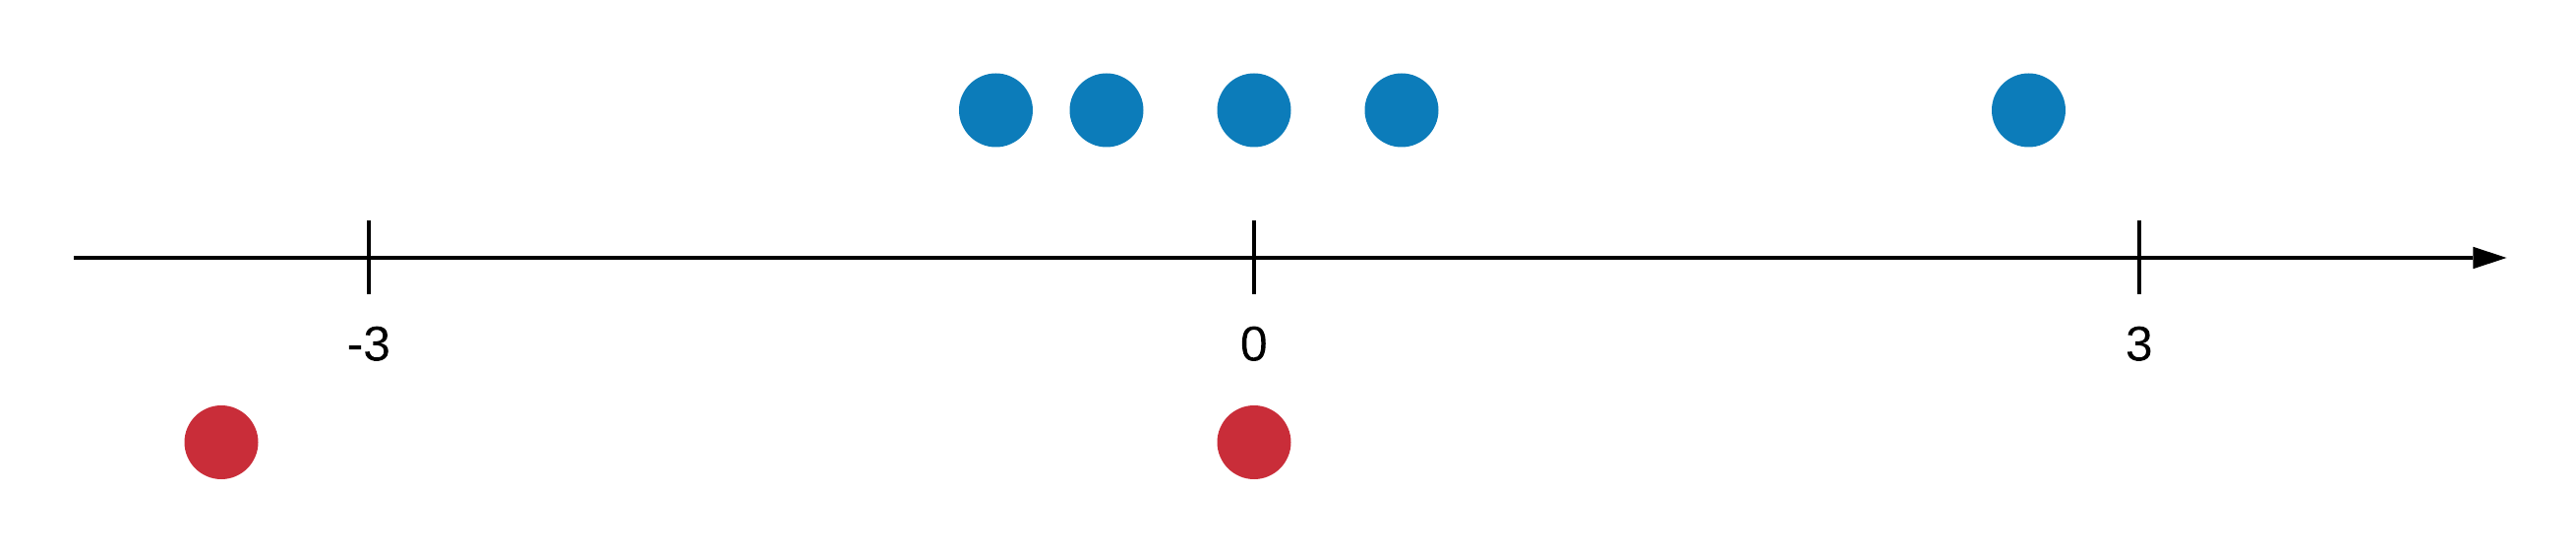
\includegraphics[width=3.5in]{./images/cut_off}
  \caption{Unwanted split at -3. Blue points represent actual data, red points synthetic data}
  \label{zero}
\end{figure}

\subsubsection{Flexible amount of synthetic data}
Instead of having exactly as much synthetic as real data in every node, we decide to allow for a certain flexibility \cite{Kruber2019UnsupervisedAS}. The number of synthetic points are still connected to the number of real data points, but the ratio may vary. We calculate based on equation \ref{equ-num}, where the $M_{S,l}(z)$ and $M_{S,r}(z)$ represent the number of synthetic points of the left and right child of $t$ respectively, assuming a split at $z$. $M_D(t)$ is the number of real data points of node $t$ and $\textrm{Pr}_t$ is the CDF of the distribution chosen for node $t$.
\begin{equation}\label{equ-num}
\begin{split}
M_{S, l}(z) & = M_{D}(t) \textrm{Pr}_t(\textrm{Z} \leq z) \\
M_{S, r}(z) & = M_{D}(t) - M_{S, l}(z)
\end{split}
\end{equation}
The number of synthetic points that node $t$ passes to its children still matches the number of data points, but they are not equally divided. The reasoning is that, if at some point we split a valid cluster close to the edges of the interval, the corresponding node will get few synthetic points and thus be almost pure. This discourages subsequent splits of that node as the Gini gain will be marginal if at all.\\


The effect of all these changes is that we have increased the average number of splits per DT from 5 to 15 and even 50 with a Gini gain of 0.05 and 0.01 respectively. When looking at the features picked for splitting, the most frequent ones are consistent over multiple runs which indicates that the URF has indeed found some structure. On the downside, the distance matrix still reports low similarities between any scenarios. This could, however, also be a result of the feature set. Regardless, considering the number of hyper parameters our model has, additional testing is required to conclude what the optimal values are.

\section{Clustering}
\label{section:clustering}
After generating a distance matrix, we run classical clustering methods on it. Unlike the URF in section \ref{section:forest}, where we needed a custom implementation because of the synthetic data at each split, we use the Scikit-learn library \cite{sklearn_api} for the clustering algorithms, because of its efficiency and flexibility.  Our implementation packages everything in a command line interface which makes it easy to switch between three different clustering techniques and adjust their parameters:
\begin{itemize}
\item Hierarchical clustering
\item DBSCAN
\item Spectral clustering
\end{itemize}

\subsubsection{Hierarchical Clustering}
Based on \cite{Kruber2019UnsupervisedAS}, we have used Hierarchical clustering on the distance matrix. The advantages of this method of clustering are its intuitiveness and ability to specify the number of clusters. It can also easily generate a cluster map, i.e. a sorted heat map, based on its output. This allows us to decide how many clusters are in the dataset. The clusters appear as squares on the diagonal of the cluster map. Figure \ref{map-scikit} exhibits three main clusters, a large one in the middle and two smaller ones above and below.

Hierarchical clustering starts with each data point as being part of its own cluster and then progressively merges the closest clusters in order to group the data. The measure by which the closest clusters are selected in each step can differ. We focus on three metrics:
\begin{itemize}
\item \emph{complete} distance
\item \emph{single} distance
\item \emph{average} distance
\end{itemize}
In the \emph{complete} case, the distance between two clusters is defined by the maximum distance between one point from the first cluster and another point from the second one. It is less sensitive to outliers but biases towards elliptic clusters. The \emph{single} case is similar, but takes the minimum distance. This makes it more susceptible to outliers but allows for different cluster shapes. The \emph{average} case, as the name implies, takes the average distance between all the points of the two clusters. Regarding its properties, it is a mix of the above two, being less sensitive to outliers than single distance and preferring elliptical clusters.

\begin{figure}[!h]
  \centering
  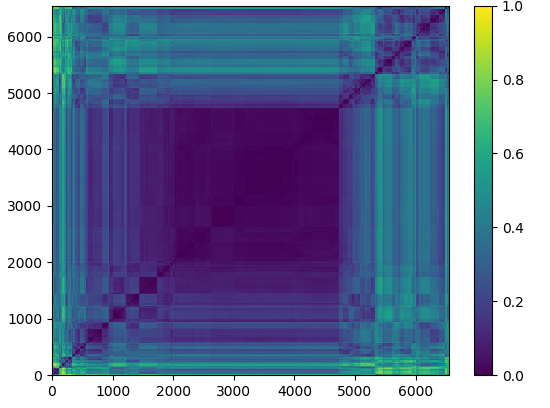
\includegraphics[width=3.5in]{./images/heatmap2}
  \caption{Cluster map generated from the DHW dataset using the Scikit-learn implementation of RF with 20000 synthetic data points, average distances}
  \label{map-scikit}
\end{figure}

\subsubsection{DBSCAN}
DBSCAN is a density based approach that has two parameters, a radius \emph{epsilon} and a number of neighbors.
\begin{equation}\label{equ:dbscan}
\begin{split}
V(p) & =\{ x \in \mathcal{D} | \ \lVert p - x \rVert \leq e\}, \ p \in \mathcal{D} \\
\mathcal{C} & = \{ p \in \mathcal{D} | \ \left| V(p) \right| \geq n \} \\
\mathcal{B} & = \{ p \in \mathcal{D} \setminus \mathcal{C} | \ \exists x \in \mathcal{D}, p \in V(x) \} \\\
\mathcal{U} & = \mathcal{D} \setminus (\mathcal{C} \cup \mathcal{B})
\end{split}
\end{equation}
We categorize points based on equation \ref{equ:dbscan}, where $\mathcal{D}$ is the set of data points, $e$ is epsilon and $n$ is the number of neighbors. We call $V(p)$ the vicinity of point $p$. $\mathcal{C}$ is the set of \emph{core} points, $\mathcal{B}$ the set of \emph{border} points and $\mathcal{U}$ the set of \emph{unlabeled} points. Unlabeled points are disregarded and are not assigned to any cluster. For core and border points, construct edges to the points in their vicinity, thus obtaining a graph. The connected components of core points form clusters. The border points are assigned to whichever cluster they have more edges.

The advantage of DBSCAN is that it performs well, regardless of the shape of the clusters. It is also very robust to outliers, thanks to the unlabeled points. In theory, this allows for a post filtering of traffic scenarios that were wrongly added to the dataset. A disadvantage of DBSCAN is its sensitivity to the relative densities of different overlapping clusters. Although good on paper, we found it difficult to apply DBSCAN on our distance matrix. The large values in the matrix forces a very narrow window for the radius and number of neighbors, mostly leading to all the points being unlabeled or all of them in the same cluster. Note that DBSCAN does not allow the user to set the number of clusters.

\subsubsection{Spectral clustering}
Spectral clustering works on a wide range on data distributions and is highly flexible. A detailed explanation of algorithm is beyond the scope of this report, but we give a brief overview. The data is first transformed into a graph, by means of k-Nearest neighbors, for instance. The diagonal degree matrix contains the degree of node $i$ on position $(i,i)$. The Laplacian matrix is build by subtracting the adjacency matrix from the degree matrix. Principal component analysis is applied to the Laplacian, reducing the dimensionality. Finally, k-Means is performed on the transformed space.

Spectral clustering allows for the number of clusters to be specified and has no restrictions concerning cluster shapes. In contrast to the other two methods, it works on the affinity matrix and not the distance matrix. We compute the affinity matrix by subtracting the distance matrix from an all one matrix. We found that spectral clustering provided similar performance to hierarchical clustering, with respect to the silhouette coefficient, even though the silhouette coefficient prefers globular clusters.

\subsection*{Silhouette coefficient}
The silhouette coefficient (SC) provides a metric to evaluate the performance of a clustering algorithm. As we don't have any labels, we can't have a traditional loss function that takes into account the ground truth. The SC takes into account the distance between different clusters as well as the distance inside each cluster.
\begin{equation}\label{equ:sil}
        \begin{split}
            a(i) & = \frac{1}{\lvert C_i \rvert} \sum_{j \in C_i, j \neq i} d(i, j) \\
            b(i) & = \min_{k \neq i}\frac{1}{\lvert C_k \rvert}\sum_{j \in C_k}d(i,j)\\
            s(i) & = \frac{b(i) - a(i)}{\max\{a(i), b(i)\}}, \textrm{ if } \lvert C_i \rvert > 1\\
            s(i) & = 1, \textrm{ if } \lvert C_i \rvert = 1
        \end{split}
\end{equation}
In equation \ref{equ:sil}, $a(i)$ represents the average distance within a cluster, $b(i)$ the average distance to the closest cluster and $s(i)$ is the silhouette coefficient itself, for cluster $i$. Note that $-1 \leq s(i) \leq 1$. The global SC is the average over all $s(i)$. 

\begin{figure}[!h]
\centering
\subfloat[][For blue: High distance within cluster, low distance between clusters]{
	
\includegraphics[width=1.4in, height=1.1in]{./images/sminus}%
	\label{fig:silhouetteminus}
}
\hfill
\subfloat[][Low distance within clusters, low distance between clusters]{
	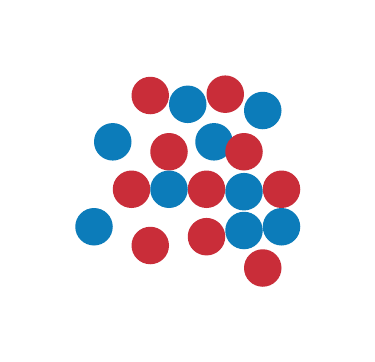
\includegraphics[width=1.4in, height=1.1in]{./images/szero}%
	\label{fig:silhouette:zero}
}
\vfill
\subfloat[][Low distance within clusters, high distance between clusters]{
	
\includegraphics[width=3.5in]{./images/sone}%
	\label{fig:silhouette:one}
}
\caption{Comparison of different clusterings with respect to the silhouette coefficient. In (a), one cluster encapsulates the other and the silhouette coefficient becomes negative for the blue points. In (b), it is around zero because the clusters overlap. In (c), it approaches 1, as the clustering is desirable. } 
\label{fig:silhouette}
\end{figure}


Figure \ref{fig:silhouette} shows the three cases of the SC, negative, around zero and close to one. Note that Figure \ref{fig:silhouetteminus} might be a desirable clustering by other measures, but the SC gives it a bad score (the global SC is, however, improved by the red group). The SC biases towards globular clusters. Because of this reason, it does not serve as a good comparison between different clustering approaches. It may, however, be used to compare between different parameters for the same method. Another downside is that it does not take into account the number of samples in a particular cluster. This lead, in our experience, to undesirable results, as it could happen that an instance in which one cluster contained most of the samples was rated better than another more balanced instance. This is not to say that we expect the results to be balanced, but the unbalance was so extreme, that most clusters only had one sample.

\section{Evaluation}
\label{section:evaluation}
\subsection{Methodology}
We performed tests on all 'Small' datasets, which contained about 6500 to 7000 samples. The forests contained 200 trees, with minimum Gini gain between 0.05 and 0.01. The maximum number of samples in leaf nodes was set to 20, 40 and 60. Note that the splitting may also stop due to insufficient Gini gain. When splitting, we forced a minimum number of 5 or 10 samples to each child, to avoid extremely unbalanced splits. The maximum depth of the trees was capped at 10. For every dataset we performed 4 runs, with 4 different subsets of features (TTC, DHW, THW and all features). For every distance matrix we performed 30 Hierarchical clusterings, 10 for every distance metric (single, average and complete), with the number of clusters ranging from 3 to 12. We ran the URF training and distance matrix calculations on 4 threads. The clustering was performed on a single thread. The entire process took around 4 hours. Afterwards, we evaluated our results based on the silhouette index, generated box plots of the most important features and looked at visualizations of 10 scenarios from each cluster, in an attempt to identify high level maneuvers.

\subsection{Results}
The best results, judged by the silhouette coefficient (SC), were achieved on the DHW dataset using all the available features. It registered a silhouette coefficient of 0.065 for average distances on three clusters. Upon closer inspection, the cluster map only showed 2 clusters (Figure \ref{map-dhw}). Another run with 2 clusters saw the SC increase to 0.071.

\begin{figure}[!h]
  \centering
  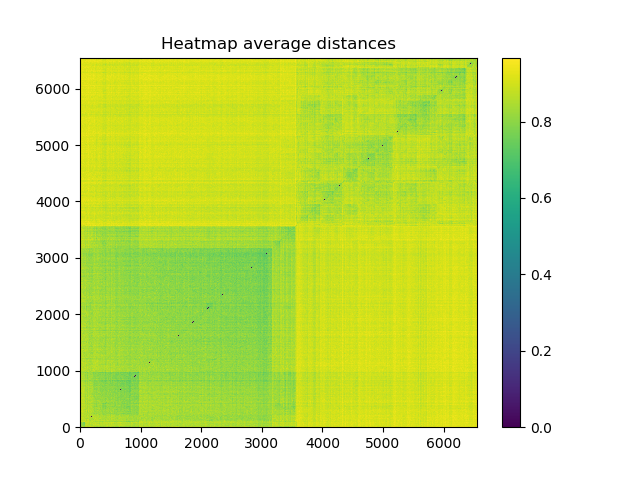
\includegraphics[width=3.5in]{./images/heatmap_dhw_all_2_avg}
  \caption{Cluster map generated from the DHW dataset. Numbers represent distances, the lower the number, the more similar the scenarios are.}
  \label{map-dhw}
\end{figure}

As to be expected from Figure \ref{map-dhw}, the silhouette coefficient kept decreasing with higher number of clusters. The differences between the various clustering methods and the number of clusters were negligible, all ranging from 0 to 0.07. We can also see from the heat map, that the scenarios recognized as similar at all, with a minimum distance of around 0.6.

By looking at the number of splits performed on each feature, we can say which features have a higher significance. Although not exactly the same among all datasets, the top features have always been related to the acceleration, breaking time or velocity of the ego vehicle at different times. Features regarding neighbors have been used less often.

\begin{figure}[!h]
  \centering
  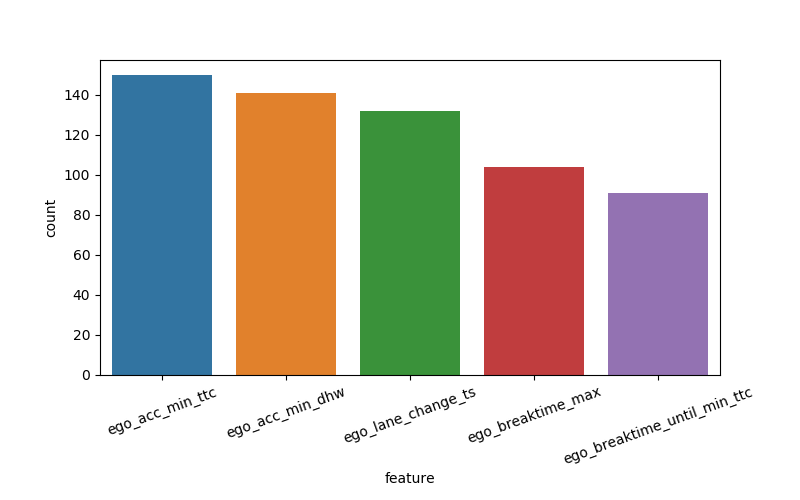
\includegraphics[width=3.5in]{./images/features_plot}
  \caption{Most used features on the DHW dataset}
  \label{map-dhw}
\end{figure}

Using this information we can plot the values of features for the different clusters. In Figure \ref{fig:boxplots:ttc}, for instance, we can see that the ego vehicle in cluster one doesn't brake until the moment of minimum TTC at all, whereas in cluster zero it does. Similarly, the ego vehicle of cluster one does not accelerate at the moment of minimum DHW, whereas it has much higher variance in cluster zero (Figure \ref{fig:boxplots:dhw}).

When looking at visualizations of the clusters, we couldn't discern any particularities of the two clusters. We believe this is in part due to the distance matrix but it may be a problem of the features as well. We also ran the library implementation of Random Forests from Scikit-learn, where the scenarios were considered much more similar to another and this yielded a much higher silhouette coefficient (around 0.5). The clusters, however, didn't seem alike to the human eye. Due to memory limitations, 20000 synthetic points were added to the around 7000 samples. This is in no way enough to uniformly cover the entire space and is exactly the reason we opted for a custom implementation of URFs.

\begin{figure}[!h]
\centering
\subfloat[][Box plot of the acceleration at minimum DHW]{
	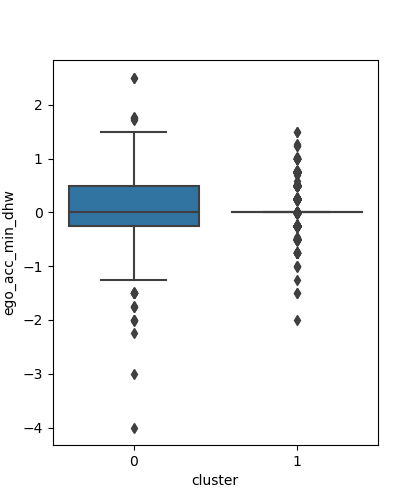
\includegraphics[width=2in]{./images/boxplot_ego_acc_min_dhw}%
	\label{fig:boxplots:dhw}
}
\hfill
\subfloat[][Box plot of the brake time until minimum TTC]{
	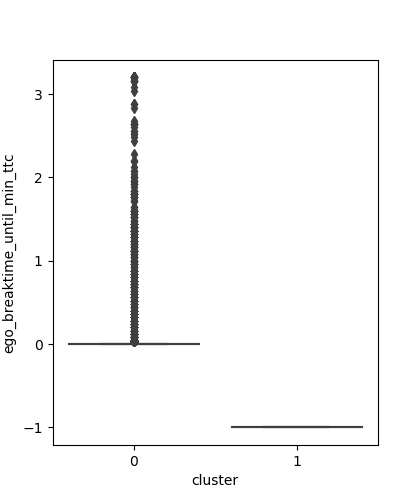
\includegraphics[width=2in]{./images/boxplot_ego_breaktime_until_min_ttc}%
	\label{fig:boxplots:ttc}
}
\caption{Values of the important features (based on the number of splits) in the clusters} 
\label{fig:boxplots}
\end{figure}

\section{Conclusion and Future Work}
\label{section:conclusion}
This paper presents an attempt to cluster freeway traffic scenarios from the highD dataset into typical driving maneuvers one would perform in such conditions. Around 60 features that characterize a driving scenario were considered, containing information about the dynamics of the ego vehicle and its six closest vehicles. The URF appears to be an appealing choice for such a task, given the high dimensionality of the data, but it proves very difficult to achieve meaningful results. This is due, in part, to the large number of hyper-parameters the model has and its lack of robustness. We explored the effect of various alterations of the URF algorithm from an empiric, intuitive and sometimes even mathematical perspective. It is our hope that our conclusions will help bring further improvements to traffic scenario clustering tasks. We have created an automated testing pipeline that facilitated large scale testing with high flexibility, as a result of many adjustable parameters. We have also created practical ways to visualize the results, by means of animations and plots.

Other clustering approaches should, however, also be considered. The complexity of the features is another area worth investigating, especially how low level features compare to high level ones under the same algorithm. Furthermore, investigating the highD dataset in order to create more balanced and robust scenario samples, as well as including other data sources in order to have wide variety of scenarios can be considered for future work.


% references section

% can use a bibliography generated by BibTeX as a .bbl file
% BibTeX documentation can be easily obtained at:
% http://www.ctan.org/tex-archive/biblio/bibtex/contrib/doc/
% The IEEEtran BibTeX style support page is at:
% http://www.michaelshell.org/tex/ieeetran/bibtex/
%\bibliographystyle{IEEEtran}
% argument is your BibTeX string definitions and bibliography database(s)
%\bibliography{IEEEabrv,../bib/paper}
%
% <OR> manually copy in the resultant .bbl file
% set second argument of \begin to the number of references
% (used to reserve space for the reference number labels box)
\bibliography{ref}
\bibliographystyle{IEEEtran}


% that's all folks
\end{document}


